\chapter{Theorie}
\label{cha:Theorie}
$\gamma$-Spektroskopie beschäftigt sich allgemein mit der Interaktion von $\gamma$-Quanten mit Materie. Damit solche Wechselwirkungen wissenschaftlich untersucht und erforscht werden
können ist es grundlegend notwendig zu wissen, welchen $\gamma$-Strahler in welchen Wellenlängen emmitieren, also kurzgefasst das Spektrum eines Strahlers zu kennen. Dazu wurden 
und werden Detektoren konstruiert, welche genau diese Spektren messen sollen. In diesem Versuch ist der Germanium Detektor von Interessse. Um zu verstehen, wie dieser Detektor 
ein Spektrum misst ist es notwendig die fundamentalen Licht-Materie-Wechselwirkungen zur verstehen. Dabei dominieren für $\gamma$-Quanten allerdings schon einige wenige.

\section{Licht-Materie-Wechselwirkungen}
\label{sec:WW}
Trifft ein Photon beliebiger Energie $E = \mathrm{h}\nu$ auf einen Atom können eine hand voll Effekte auftreten. Dabei existieren drei verschiedene Interaktionspartner in einem Atom. 
Das Photon kann entweder mit Elektronen, dem Kern oder dem elektrischen Feld des Atoms wechselwirken. Bei jeder Wechselwirkung (WW) können drei unterschiedliche \enquote{Endzustände}
für das Photon auftreten. Es kann annihiliert oder gestreut werden. Bei der Streuung werden zwei fälle unterschieden. Es kann elastisch oder inelastisch gestreut werden. 
In der Tabelle in Abbildung \ref{fig:WW_photon} werden (fast) alle möglichen Wechselwirkungsprozesse genannt.

\begin{figure}
    \centering
    \includegraphics[width = \textwidth]{content/pics/tabelleGamma.png}
    \caption{Darstellung der möglichen Licht-Materie-Wechselwirkungsprozesse.}
    \label{fig:WW_photon}
\end{figure}

Dabei hängt es von der Energie des einfallenden Photons und vom \enquote{Zufall} ab welcher Prozess stattfindet. Zufall meint dabei, dass das Geschehniss statistisch verteilt ist und 
lediglich eine Abschätzung/Bestimmung der Wahrscheinlichkeit Aufschluss darüber gibt wie die Häufigkeit der Prozesse verteilt ist. Ein Maß für diese Wahrscheinlichkeit ist der
Wirkunsquerschnitt (WQ) $\sigma(E)$. Im Germanium Detektor sollen $\gamma$-Quanten gemessen gemessen werden. Für diesen Spektralbereich und im Falle von Germanium, welches die Ordnungszahl
$Z = 32$ hat, ist der gesamte Extinktionskoeffizient in Abbildung \ref{fig:germanium_wq} dargestellt. 

\begin{figure}
    \centering
    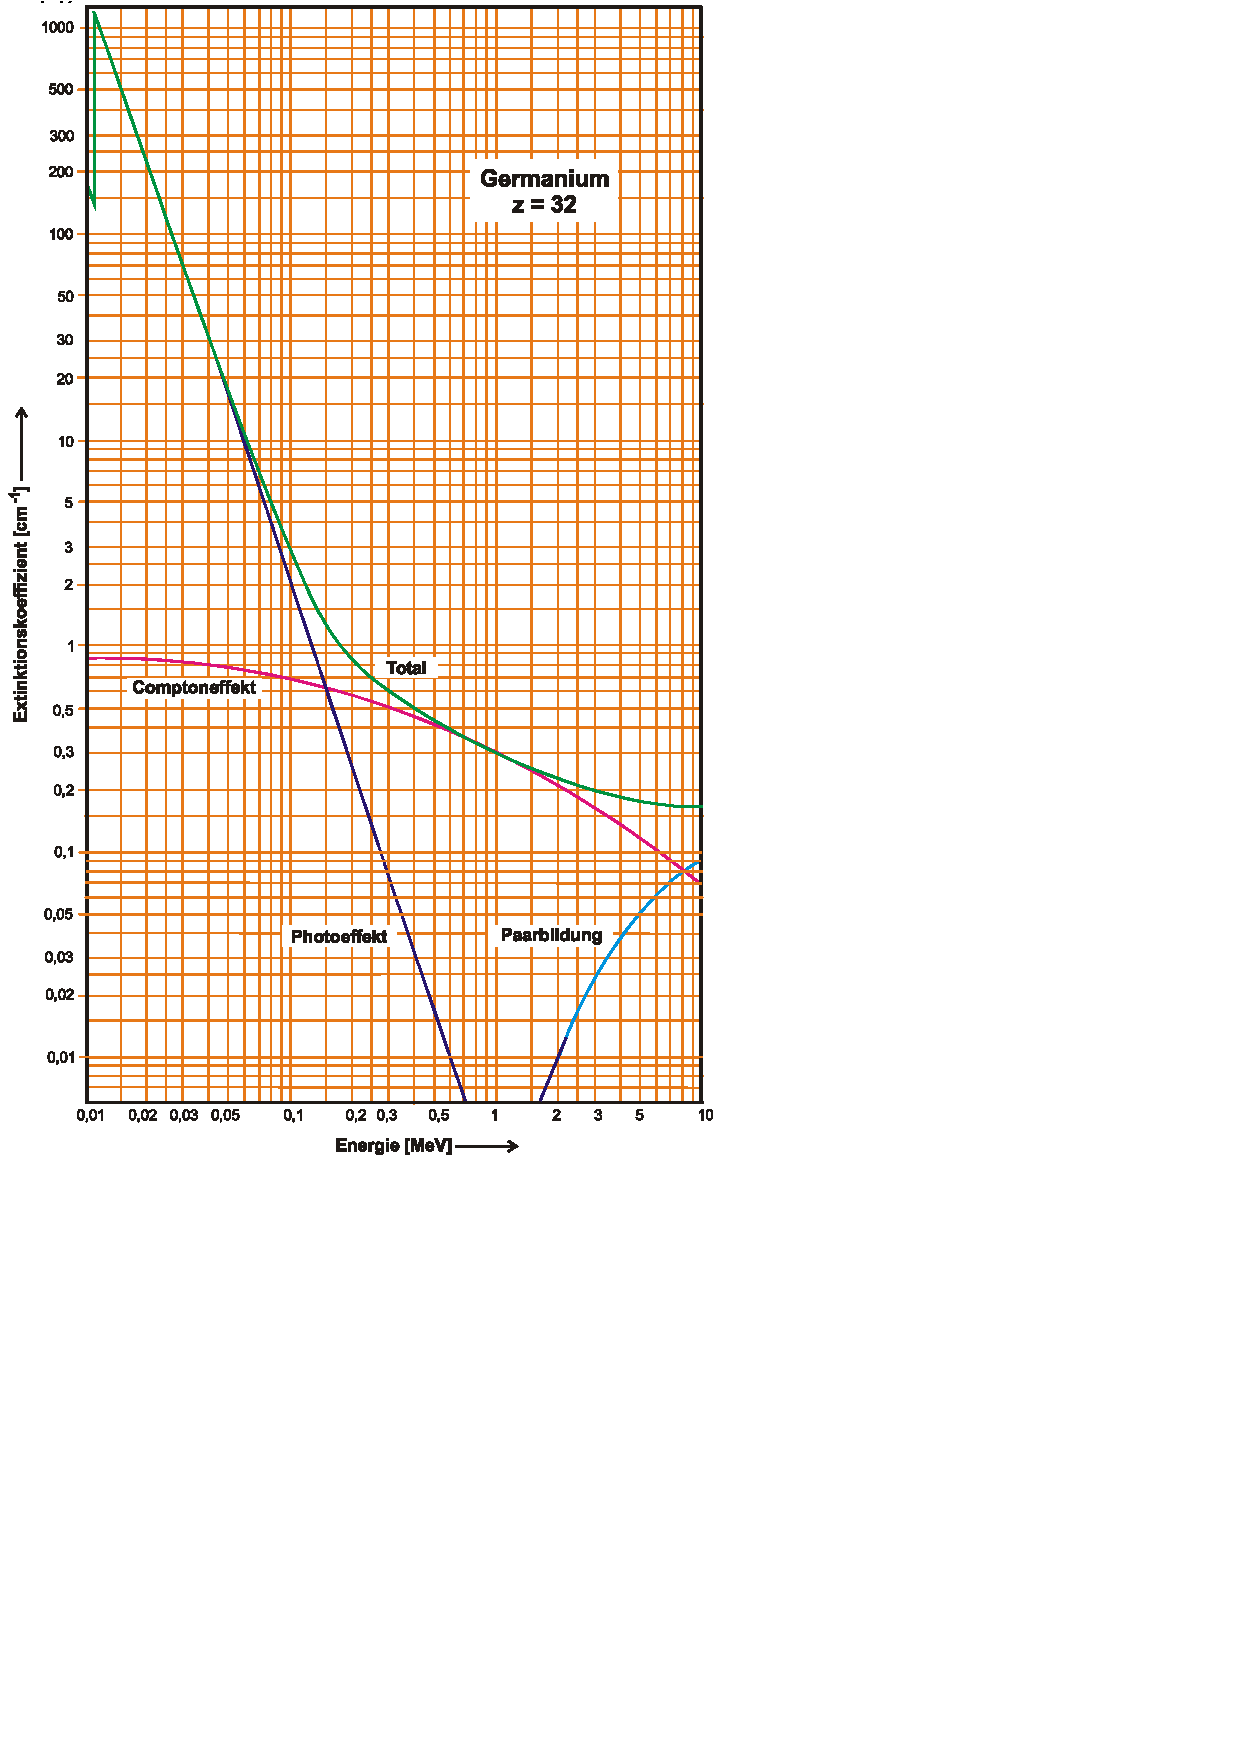
\includegraphics[height = \textheight]{content/pics/wq_germanium.pdf}
    \caption{Totaler Wirkunsquerschnitt von Germanium.}
    \label{fig:germanium_wq}
\end{figure}

Wie in Abbildung \ref{fig:germanium_wq} gezeigt, dominieren für $\gamma$-Quanten drei Effekte. Der Photoeffekt, Compton-Effekt und die Paarbildung, welche dann durch überlagerung 
den totalen WQ ergeben. Dies bedeutet, dass die anderen genannten Effekte vernachässigbar klein sind und im WQ gar nicht betrachtet werden. In diesem Versuch werden lediglich 
Strahler verwendet, welche ein Spektrum bis zu $\qty{1}{\mega\electronvolt}$ haben. Daher kann für diesen Versuch die Paarbildung ignoriert werden. Es finden also maßgeblich 
zwei Effekte statt.

\subsection{Photoeffekt}
\label{subsec:photoeffekt}
Wie Abbildung \ref{fig:WW_photon} zu entnehmen ist wird das Photon bei diesem Prozess vollständig annihiliert. Dabei transferiert es seine gesamte Energie an das Elektron.
Beim äußeren Photoeffekt interagiert das Photon mit einem Valenzelektron. Der Energieübertrag des Photons muss mindestens gleich der Bindungsenergie des Elektrons sein, sodass 
das Elektron aus der Schale herausgelößt wird. Die restliche Energiedifferenz $\Delta E = E_{\gamma} - E_{\mathrm{B}}$ erhält das Elektron als kinetische Energie. Dabei ist 
$E_{\gamma}$ die Energie des Photons und $E_{\mathrm{B}}$ die Bindungsenergie der Schale des Elektrons. Tritt nun aber der innere Photoeffekt auf, das heißt es wird nicht das 
äußere Valanzelektron, sondern ein Elektron der inneren geschlossenen Schalen ausgelöst, verbleibt ein Loch in jener Schale. Da sich das Atom in den energetisch günstigsten 
Zustand begeben wird, fällt ein äußeres Elektron in dieses Loch zurück. Dabei wird die Differenzenergie der Schalen als Photon emittiert. Dieses Photon kann natürlich auch 
wieder wechselwirken, allerdings hat es eine geringere Energie als das \enquote{erste} Photon. Nachdem durch den Photoeffekt ein Elektron ausgetreten ist und sich mit seiner
kinetischen Energie durch den Detektor bewegt, kann es weitere Elektronen durch Stöße anregen. Bei einer solchen Anregung treten die Elektronen von ihrem Valanzband in das 
Leitungsband. Durch die Wechselwirkungen wird beim Photoeffekt fast die ganze Energie im Detektor deponiert. Gerade im Germanium Detektor ist der Photoeffekt relevant, da der WQ
$\propto Z^3$ ist. Da der Photoeffekt die Qualität des Detektors stark anhebt, ist Germanium besser geeignet als Silizium, obgleich dieses günstiger wäre.

\subsection{Compton-Effekt}
\label{subsec:comptoneffekt}
Beim Compton-Effekt handelt es sich um eine inelastische Streuung an einem quasi-freien Elektron. Das Photon gibt dabei einen Teil seiner Energie an das Elektron ab und ändert 
seine Ausbreitungsrichtung. Ein einfallendes Photon der Energie $E_{\gamma}$ hat nach der Compton-Wechselwirkung die Energie 

\begin{equation}
    \label{eqn:E_compton}
    E_{\gamma}' = E_{\gamma}\frac{1}{1+\epsilon(1-\cos(\theta))}.
\end{equation}

Dabei ist $\epsilon = \sfrac{E_{\gamma}}{m_{\mathrm{e,0}}c^2}$ und $\theta$ der Streuwinkel des Photons. Die Energie des Elektrons ergibt sich aus 
\begin{equation}
    \label{eqn:E_elek_compton}
    E_\mathrm{e} = E_{\gamma} - E_{\gamma}' = E_{\gamma}\frac{\epsilon(1-\cos(\theta))}{1+\epsilon(1-\cos(\theta))}.
\end{equation}

Anhand von Gleichung \ref{eqn:E_compton} ist zu erkennen, dass der maximale Energieübertrag bei einem Streuwinkel von $\Theta = \qty{180}{\degree}$ stattfindet.
Der differentielle Wirkungsquerschnitt des Comptoneffekts ist durch 
\begin{equation}
    \label{eqn:WQ_compton}
    \frac{\mathrm{d}\sigma}{\mathrm{d}E} = \frac{3}{8}\frac{\sigma_\mathrm{Th}}{m_{\mathrm{e,0}}c^2\epsilon^2}\left(2+\left(\frac{E}{E_{\gamma} - E}\right)^2\left(\epsilon^{-2}+\frac{E_{\gamma} - E}{E}-\frac{2}{\epsilon}\left(\frac{E_{\gamma} - E}{E}\right)\right)\right).
\end{equation}

Dabei ist $\sigma_\mathrm{Th}$ der Thomson-Wirkungsquerschnitt.

\section{Germanium Detektor}
\label{sec:germanium_detektor}
Der grundlegende Aufbau des Germanium Detektors ist in Abbildung \ref{fig:germanium_detector} dargestellt. Die äußere Aluminiumschicht dient lediglich der Sicherheit und hat nichts 
mit dem Detektor zu tun. Der Detektor besteht aus aus einem Germanium-Kristall, welcher eine koaxiale Einkerbung besitzt. 

\begin{figure}
    \centering
    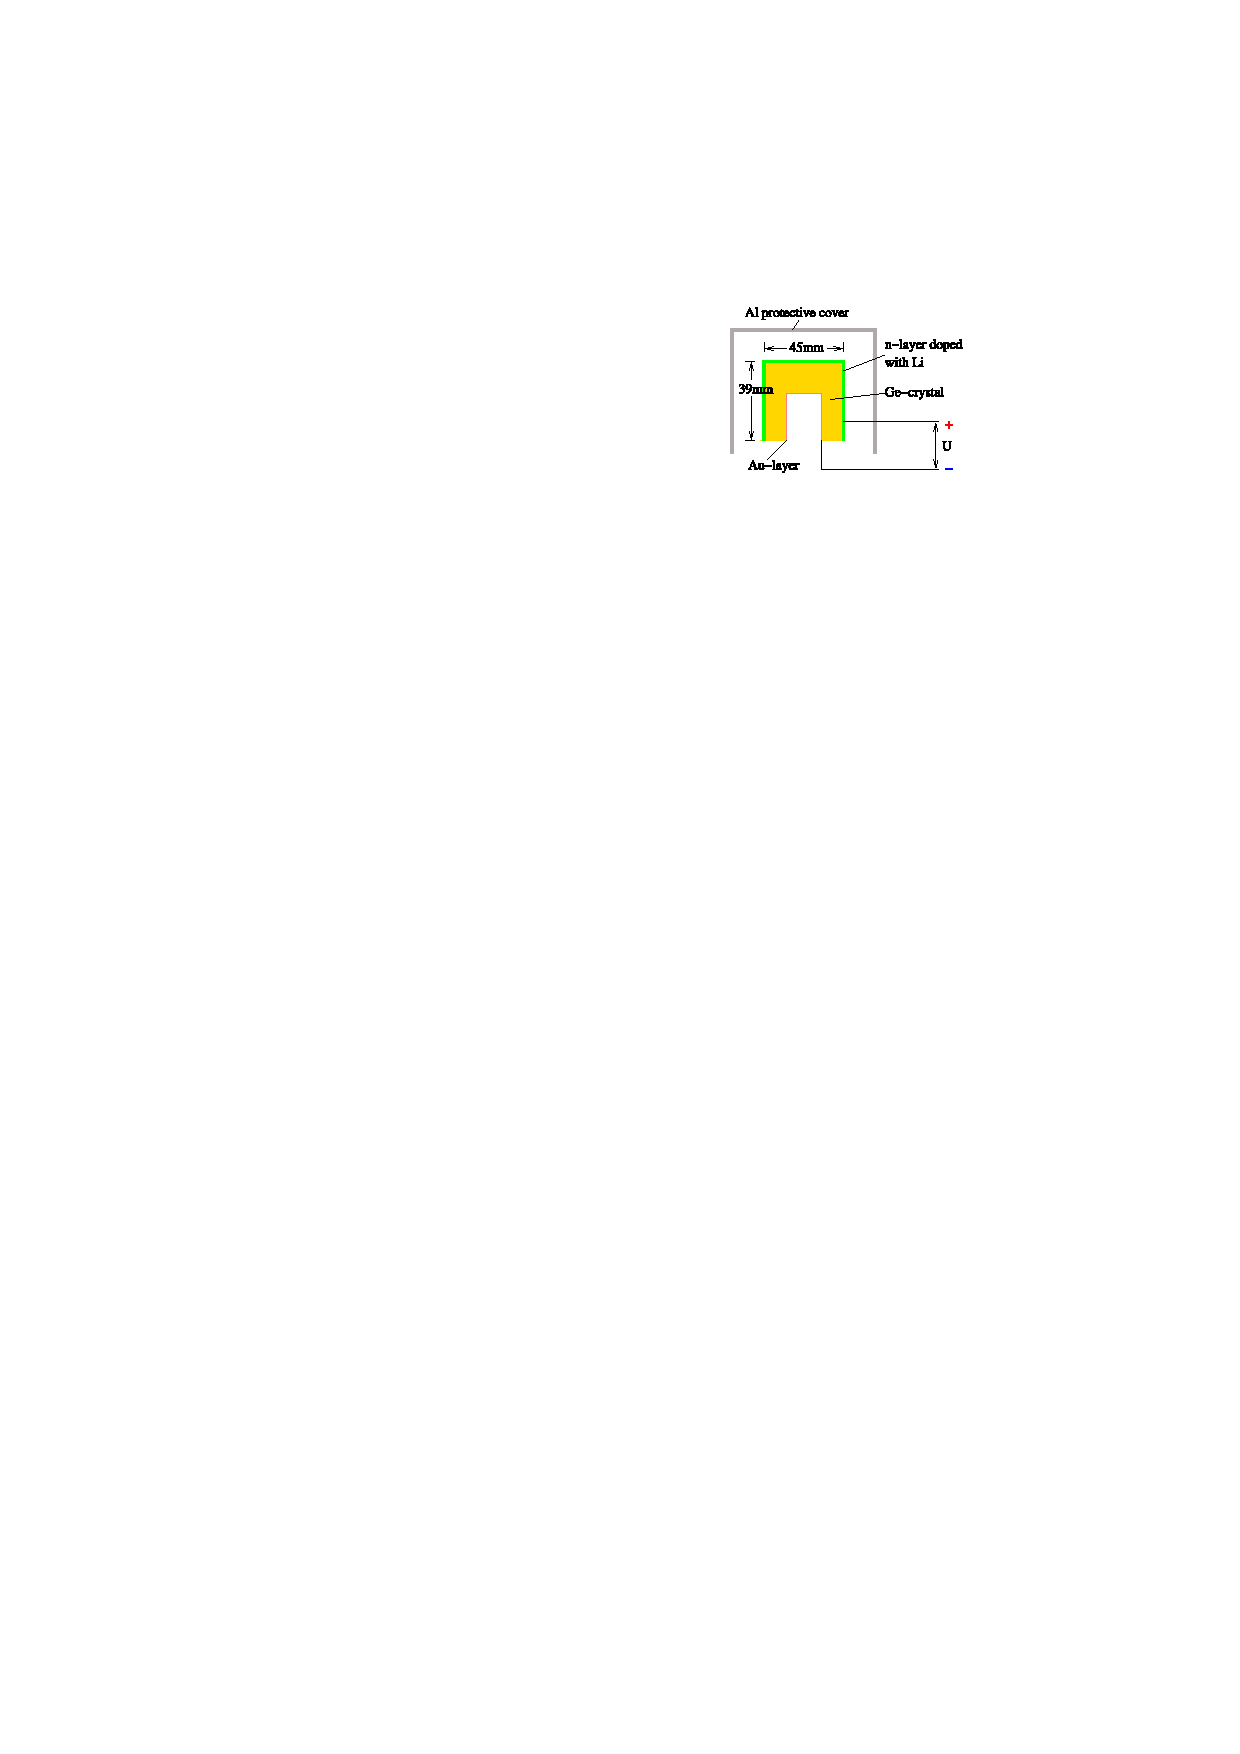
\includegraphics[width = \textwidth]{content/pics/germanium_detector_skizze.pdf}
    \caption{Schematischer Aufbau des verwendeten Germanium Detektors.}
    \label{fig:germanium_detector}
\end{figure}

Die in der Abbildung \ref{fig:germanium_detector} grün 
dargestellte Schicht ist eine aufgedampfte Lithium Schicht. Durch diese Aufdampfung entsteht eine n-dotierte Schicht am grünen Rand des Germanium-Kristalls. 
Am gegenüber liegendem Rand des Germanium-Kristalls, in der Abbildung \ref{fig:germanium_detector} in orange dargestellt, befindet sich eine dünn angebrachte Goldschicht.
Gold ist ein Metall und Germanium ist ein indirketer Halbleiter mit einer Bandlücke von $E_\mathrm{g} = \qty{0.661}{\electronvolt}$ \cite{germanium_gap}. Daher entsteht an der
Kontaktfläche von Gold und Germanium eine Metall-Halbleiter-Verbindung. Eine solche Verbindung erzielt eine starke p-Dotierung in der Nähe der Kontaktfläche. Aufgrund der 
starken Dotierung ergiebt sich zwischen den dotierten Schichten eine Raumladungszone. Diese bildet sich durch Diffundiering der reziproken Ladungsträger, welche im Gliechgewicht
ein elektrisches Feld entgegen der Dotierung erzeugen. Der Germanium-Kristall ist also ähnlich zu einer Diode aufgebaut. Nun wird zwischen der n und p Schicht eine äußere Spannung 
angelegt. Diese kann die Raumöadungszone verstärken oder annihilieren. Für den Germanium Detektor wird die Spannung in Sperrrichtung angelegt, das heißt das elektrische Feld der 
Raumladungszone wird verstärkt. Dadurch wird die Raumladungszone breiter. Der Bereich der Raumladungszone ist notwendig, um die Photonen zu detektieren. 

Trifft ein Photon in der Raumladungszone ein wechselwirkt es über die im Abschnitt \ref{sec:WW} genannten Prozesse. Durch das Photon entstehen also Elektron-Loch Paare, welche durch 
das lokal starke elektrische Feld getrennt werden bevor sie rekombinieren können. Diese Ladungsträger sammeln sich dann an den Elektroden. Diese Ladung kann dann als Spannung 
gemessen werden. Allerdings ist die Ladungsmenge pro WW klein. Daher wird ein \enquote{charge amplifier} verwendet, um das Signal zu verstärken. Ein solcher Verstärker wandelt eine 
kleine Ladungsmenge in eine verstärkte Spannung um, welche dann gemessen werden kann. Die Spannung ist dabei abhängig von der deponierten Energie des einfallenden Photons. 

Germanium hat mit $\qty{0.661}{\electronvolt}$ eine relativ kleine Bandlücke. Daher können auch schon thermische Anregungen im Detektor ausreichen um ein Signal zu erzeugen. 
Dies stellt einen großen Störfaktor da. Durch Kühlung des Detektors während der Messung lässt sich dieser Faktor beheben. Der Detektor wird mit flüssigem Stickstoff auf 
circa $\qty{77}{\kelvin}$ runtergekühlt.

\section{Spektrum eines monochromatischen Gammastrahlers im Ge-Detektor}
\label{sec:spektrum}
Ein typische Spektrum eines monochromatischen Gammastrahlers im Germanium Detektor weißt einige Eigenschaften auf. Ein solches Spektrum wird in Abbildung \ref{fig:gammaspektrum} 
dargestellt.

\begin{figure}
    \centering
    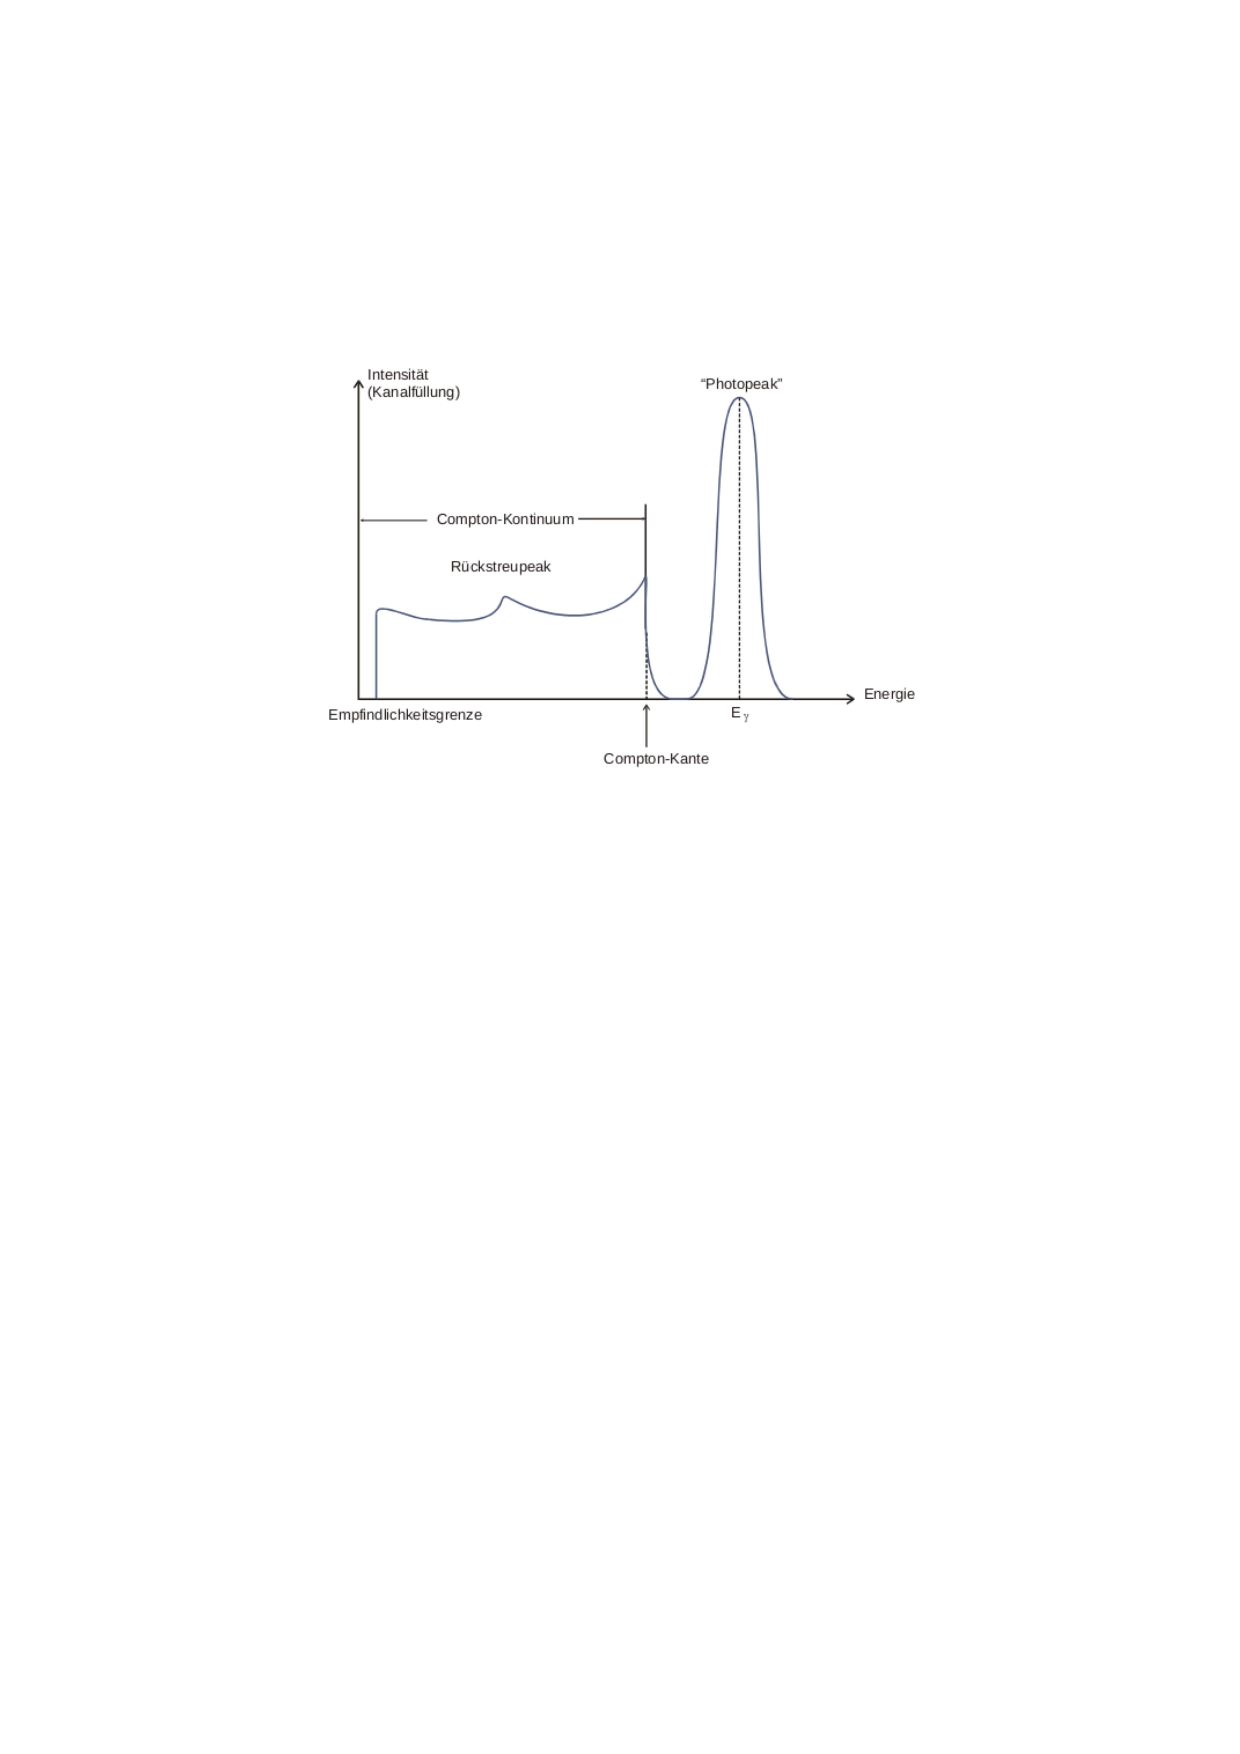
\includegraphics[width = .8\textwidth]{content/pics/gammspektrum.pdf}
    \caption{Schematisches Spektrum eines monochromatischen Gammastahlers im Germanium Detektor.}
    \label{fig:gammaspektrum}
\end{figure}

In Abbildung \ref{fig:gammaspektrum} beginnt die Intensitätverteilung erst ab einer gewissen Energieschwelle. Diese ergibt sich aus diversen experimentellen Detektoreigenschaften. 
In diesem Versuch liegt diese Schwelle bei ungefähr $\qty{40}{\kilo\electronvolt} - \qty{50}{\kilo\electronvolt}$. Bei steigender Energie bildet sich dann zunächst das 
Compton-Knotinuum. Dieses ist ein kontinuierliches Spektrum, da der Energieübertrag des Photons nicht diskret ist, sondern kontinuierlich vom Struwinkel abhängt. Innerhalb des 
Kontinuums liegt der Rückstreupeak. Dieser entsteht, da der Gammastrahler nicht nur in eine Richtung strahlt, sondern konzentrisch. Daher können die Photonen auch erst von außerhalb 
des Detektors durch Comptonstreuung zum Detektor gelengt werden. Dieser Streueffekt sorgt für höhere Zählraten mit einem Peak, dem Rückstreupeak. Der Rückstreupeak kann Abgeschätzt 
werden, indem die Compton-Energie für den Streuwinkel $\Theta=\qty{180}{\degree}$ ausgewertet wird. 
\begin{equation}
    \label{eqn:Rückstreupeak}
    E_ = E_{\gamma}\frac{1}{1+2\epsilon}
\end{equation}

Das Compton-Kontinuum endet mit einer maximalen cutoff Energie, der Comptonkante. Diese liegt bei der hälfte das Abfalls nach dem letzten Peak. Die Energie der Comptonkante 
$E_\mathrm{max}$ berechnet sich aus 
\begin{equation}
    \label{eqn:comptonkante}
    E_\mathrm{max} = E_{\gamma}\frac{2\epsilon}{1+2\epsilon}.
\end{equation}

Danach befindet sich im Energiespektrum der Photopeak. Der Photopeak, oder auch full energy peak genannt, beinhaltet die gesamte Energie des einfallenden Photons. Dieser Peak resultiert
alleinig aus dem Photoeffekt. 

\section{Kenngrößen des Germanium Detektors}
\label{sec:Kenngroessen}
Eine wichtige Kenngröße des Germanium Detektors ist die Halbwärtsbreite das Photopeaks. Diese Kenngröße definiert das Energieauflösungsvermögen des Detektors. Daher gibt diese 
Kenngröße an, ob zwei Energie-Peaks in einem Spektrum unterschieden werden können oder nicht. Diese Kenngröße unterliegt allerdings auch materialbedingten Störungen. Um diese 
zu minimieren muss eine passende Spannung angelegt werden. 

Einer weitere wichtige Kenngröße ist die Effizienz. Diese beshreibt die Detektionswahrscheinlichkeit abhängig von der Energie. Diese ist charakteristisch für einen Detektor.

